%\addcontentsline{toc}{chapter}{Development Process}
\chapter{Design}
	There are 2 main parts of the project the first being the server element and the second the mobile application itself. The mobile application will be connecting to the server applications through a RESTFull API to retrieve all of the data that's required. The server element will be composed of 3 main parts the RESTFull API, Administration panel, and the data mining part.
	\begin{figure}[ht] % H - For exact position 
			\caption[Overview design]{This diagram shows the main areas of the project and how the interact with each other. }
			\centering
			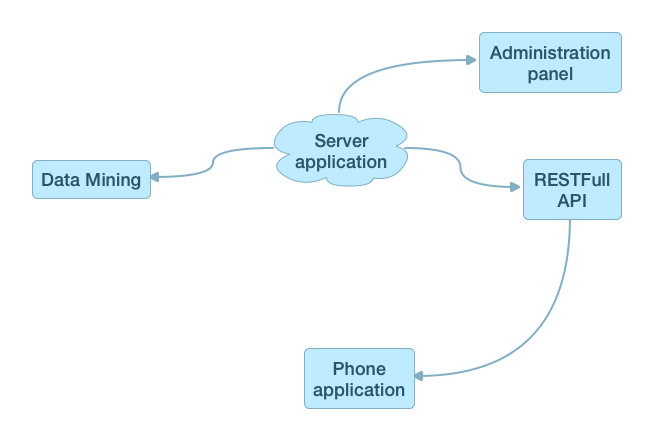
\includegraphics[width=0.5\textwidth]{Images/overview-design}
			\label{fig:overview-design}
		\end{figure}
	
	\section{Database}
		To full fill the requirement of utilising a cloud server solution the database will be using PostgresSQL which the server element will interface with it using the ActiveRecord gem bundled with Ruby on Rails. Because the server element was designed using TDD and each the overall design, was moulded during the process Figure \ref{fig:erd} shows the resultant entity relationship diagram at the end of the project. There is also a set of definite fields that was worked from the Facebook API schema listed in Table \ref{fig:facebookEventVenues}, schema.org\cite{schemaEvent} was also used to help build the list of relevant information on an event. 

		\begin{figure}[ht] % H - For exact position 
			\caption[Entity Relationship Diagram]{This diagram depicts the various entities, and their interactions with each other.}
			\centering
			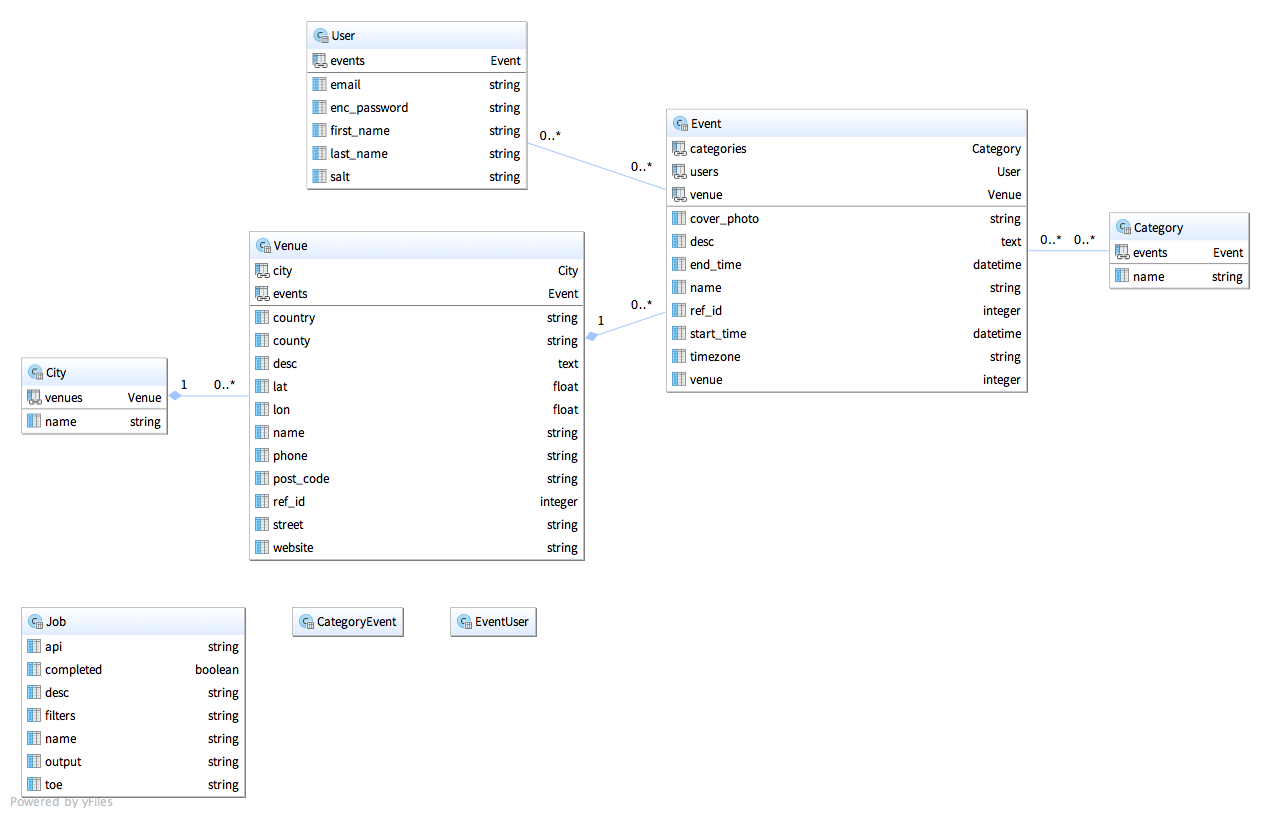
\includegraphics[width=1\textwidth,angle=90]{Images/ERD}
			\label{fig:erd}
		\end{figure}

	\section{Server Application}
		The server application, will be composed of 3 components these will be the Data mining module, the RESTFull API for interfacing with the mobile application, and the administration panel. These components whilst being separate, will all interact with the same database and will reside within the same code base to be uploaded and ran on the cloud application platform (CAP).

		\subsection{Development tools}
			The server application will be written in Ruby utilising the Ruby on Rails (RoR) framework, there were other options to use such as; Node, Clojure, Java, Python. However the RoR framework provided great native support for developing API's and database integration. Rails also gives us the ability to run code using the rails environment via the command line by use of rake tasks. The CAP will call the task hourly using a cron job to pull in new events and venues, these jobs will be specified by the administration panel and then ran by the rake task. 

			To develop the server side code the programmer will be using the Sublime Text 2 text editor\cite{sublime} with the following packages installed; RSpec\cite{RSpecSub}, Ruby Test\cite{RubyTest}, and Rails Developer Snippets\cite{RDS}. These packages will assist the programmer by allowing them to run tests within the editor and provide key snippets to be used by them. The use of a text editor with the packages noted installed allowed a cleaner interface for the programmer to deal with and was a tool they where familiar with. 

			As stated above, the programmer will be following a test driven development approach as such it will be required to use some form of test framework. For this the programmer will be using RSpec for RoR gem\cite{RSpecRails}, this gem provides the user with the RSpec suite correctly optimised and set-up to be used within a RoR environment. The programmer will also be using FactoryGirl\cite{FactoryGirl} a higher grain of control over mock models, and WebMock\cite{WebMock} to be able to mock API connections with test data. 

		\subsection{OAuth}
			The application will use the OAuth standard for authentication to the application, OAuth is an open protocol that offers `secure client delegation'. By delegating a different user token for each user the server can serve user specific data to each user, whilst ensuring statelessness. The use of OAuth will also restrict server resources to defined applications, allowing a higher level of control to the applications that utilise the API. 

		\subsection{Routes}
			Ruby on Rails allows for a series of URL routes to be defined, to ensure the project follows REST principles the API the interface is required to be uniform, for this all requests will be responded in JSON and will be in the format similar to snippet \ref{fig:JSONOutput}. The API URI structure should also be representational of the data being served and how the data is structured in the database. Table \ref{fig:apiRoutesTable} shows the endpoints and accessors for the data that's available through the API. The returned data will also be paginated using the gem api-pagination\cite{paginate} the pagination URIs will be formed as part of the header information of the response to keep the returned body easy to parse. 

			\begin{program}
				\begin{verbatim}
				{
					`code' => `201',
					`errors' => `',
					`body' => [ ]
				}
				\end{verbatim}
				\caption{Example JSON output for REST requests}
				\label{fig:JSONOutput}
			\end{program}

			\begin{table}[h]
				\centering
				\caption{API Routes}
				\begin{tabular}{|l|l|l|}
				\hline
				Verb &  URI Pattern                                      &  Controller\#Action                           \\ \hline
				GET  &    /api/v1/events(.:format)                       &                     api/v1/events\#index      \\
				GET  &    /api/v1/events/:id(.:format)                   &                 api/v1/events\#eventByID      \\
				GET  &     /api/v1/venues(.:format)                      &                      api/v1/venues\#index     \\
				GET  &     /api/v1/venues/:id(.:format)                  &                  api/v1/venues\#show          \\
				GET  &     /api/v1/venues/:id/events(.:format)           &           api/v1/events\#eventsByVenue        \\
				POST &    /api/v1/register(.:format)                     &                    api/v1/user\#register      \\
				GET  &     /api/v1/user(.:format)                        &                        api/v1/user\#index     \\
				POST &    /api/v1/user(.:format)                         &                       api/v1/user\#update     \\
				GET  &     /api/v1/user/feed(.:format)                   &                  api/v1/user\#feed            \\
				GET  &     /api/v1/user/following(.:format)              &              api/v1/following\#index          \\
				POST &    /api/v1/user/follow(.:format)                  &                 api/v1/following\#followEvent \\
				POST &    /api/v1/user/unfollow(.:format)                &               api/v1/following\#unfollowEvent \\ 
				GET  &    /api/v1/categories(.:format)                   &                  api/v1/categories\#index     \\
				GET  &     /api/v1/categories/:id(.:format)              &              api/v1/categories\#show          \\
				GET  &     /api/v1/categories/:id/events(.:format)       &      api/v1/events\#eventsByCategory          \\
				GET  &     /api/v1/cities(.:format)                      &                      api/v1/cities\#index     \\
				GET  &     /api/v1/cities/:id(.:format)                  &                  api/v1/cities\#show          \\
				GET  &     /api/v1/cities/:id/events(.:format)           &           api/v1/events\#eventsByCity         \\
				GET  &     /api/v1/cities/:city\_id/venues(.:format)     &     api/v1/venues\#venuesByCity               \\
				GET  &     /api/v1/cities/:city\_id/categories(.:format) &  api/v1/categories\#catsByCity                \\ \hline
				\end{tabular}
				\label{fig:apiRoutesTable}
			\end{table}

			% \begin{table}
			% 	\centering
			% 	\caption{OAuth Routes}
			% 	\begin{tabular}{|l|l|l|}
			% 	\hline
			% 	GET    &     /oauth/authorize/:code(.:format)           &             doorkeeper/authorizations\#show           \\ \hline
			% 	GET    &     /oauth/authorize(.:format)                 &                    doorkeeper/authorizations\#new     \\
			% 	POST   &    /oauth/authorize(.:format)                  &                    doorkeeper/authorizations\#create  \\
			% 	PATCH  &   /oauth/authorize(.:format)                   &                    doorkeeper/authorizations\#update  \\
			% 	PUT    &     /oauth/authorize(.:format)                 &                    doorkeeper/authorizations\#update  \\
			% 	DELETE &  /oauth/authorize(.:format)                    &                    doorkeeper/authorizations\#destroy \\
			% 	POST   &    /oauth/token(.:format)                      &                        doorkeeper/tokens\#create      \\
			% 	GET    &     /oauth/applications(.:format)              &                 doorkeeper/applications\#index        \\
			% 	POST   &    /oauth/applications(.:format)               &                 doorkeeper/applications\#create       \\
			% 	GET    &     /oauth/applications/new(.:format)          &             doorkeeper/applications\#new              \\
			% 	GET    &     /oauth/applications/:id/edit(.:format)     &        doorkeeper/applications\#edit                  \\
			% 	GET    &     /oauth/applications/:id(.:format)          &             doorkeeper/applications\#show             \\
			% 	PATCH  &   /oauth/applications/:id(.:format)            &             doorkeeper/applications\#update           \\
			% 	PUT    &     /oauth/applications/:id(.:format)          &            doorkeeper/applications\#update            \\
			% 	DELETE &  /oauth/applications/:id(.:format)             &             doorkeeper/applications\#destroy          \\
			% 	GET    &     /oauth/authorized\_applications/  &      doorkeeper/authorized\_applications\#index       \\
			% 	DELETE &  /oauth/authorized\_applications/:id &  doorkeeper/authorized\_applications\#destroy         \\
			% 	GET    &     /oauth/token/info(.:format)                &                   doorkeeper/token\_info\#show        \\ \hline
			% 	\end{tabular}
			% 	\label{fig:OAuthRoutesTable}
			% \end{table}
		
		\subsection{Data mining element}
			The data mining element is broken up into a 2 different parts these being the interfaces to the external data sources, and the second being the job scheduler. Figure \ref{fig:mining} shows how these parts will work together to input data from the various API's that's needed. To allow for any number of API's to be added to the system, a base class called `Resources' will be needed with any inherited functions needed Figure \ref{fig:class_api} shows the class diagram for this part of the project. Then another class that inherited from `Resources' will be used to define each individual API connection. By doing this the API is easy to extend simply by working as a interpreter to the different names for data fields and layout for each API response. The scheduler RAKE  task will then read in the jobs defined by the administration panel and pull in the relevant information and insert this into the database.

			\begin{figure}[ht] % H - For exact position 
				\caption[Class Diagram for API integration ]{This diagram describes the functions and inheritance used for the library that connects to the APIs}
				\centering
				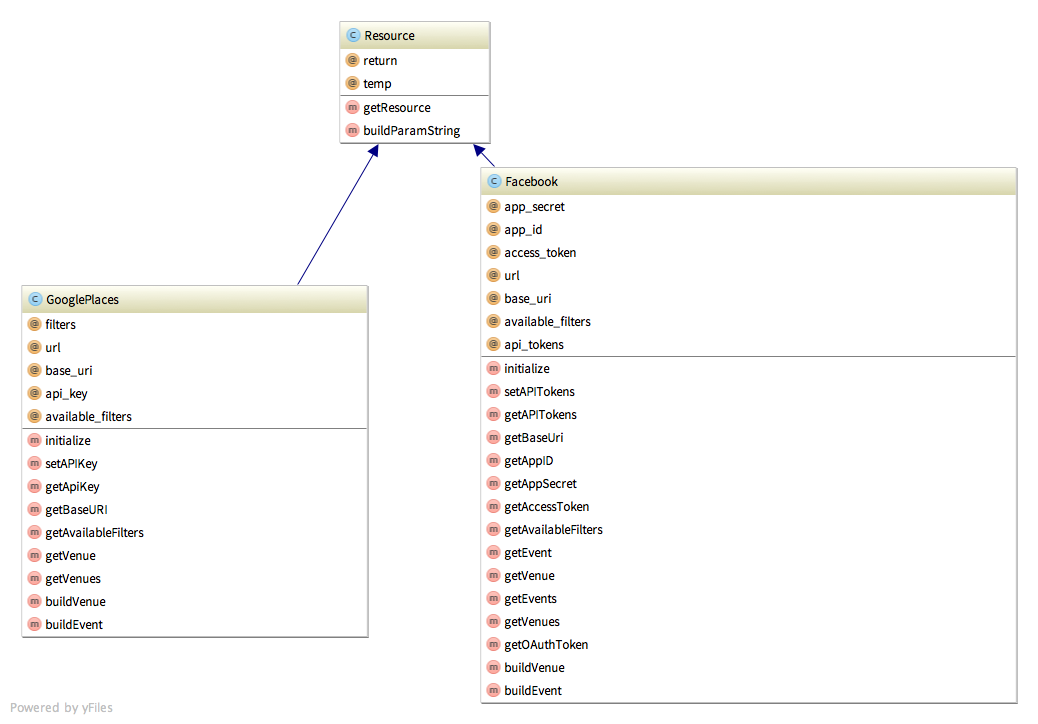
\includegraphics[width=1\textwidth]{Images/resources}
				\label{fig:class_api}
			\end{figure}

			\begin{figure}[ht] % H - For exact position 
				\caption[Overview of the data mining aspect]{This diagram shows an overview of how the different data mining module is composed.}
				\centering
				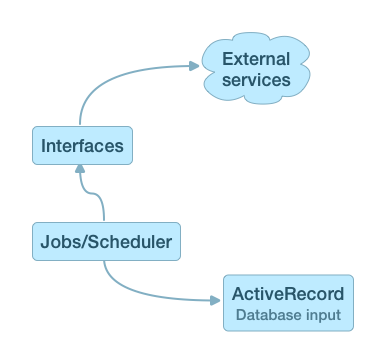
\includegraphics[width=0.5\textwidth]{Images/mining-overview}
				\label{fig:mining}
			\end{figure}

		\subsection{Class diagram}
			Following on from the MVC design pattern and the fact the API needs to be representational, each controller is representational for each table stored in the database. However in some cases there are filters such as being able to get the events via the venue, since this will return a list of events rather than venues the method to do this is inside the events controller. Figure \ref{fig:controllers} shows the structure of the controllers, and the methods inside of them. 

			\begin{figure}[ht] % H - For exact position 
				\caption[Controllers Class Diagram]{This diagram shows the classes along with the methods and class variables}
				\centering
				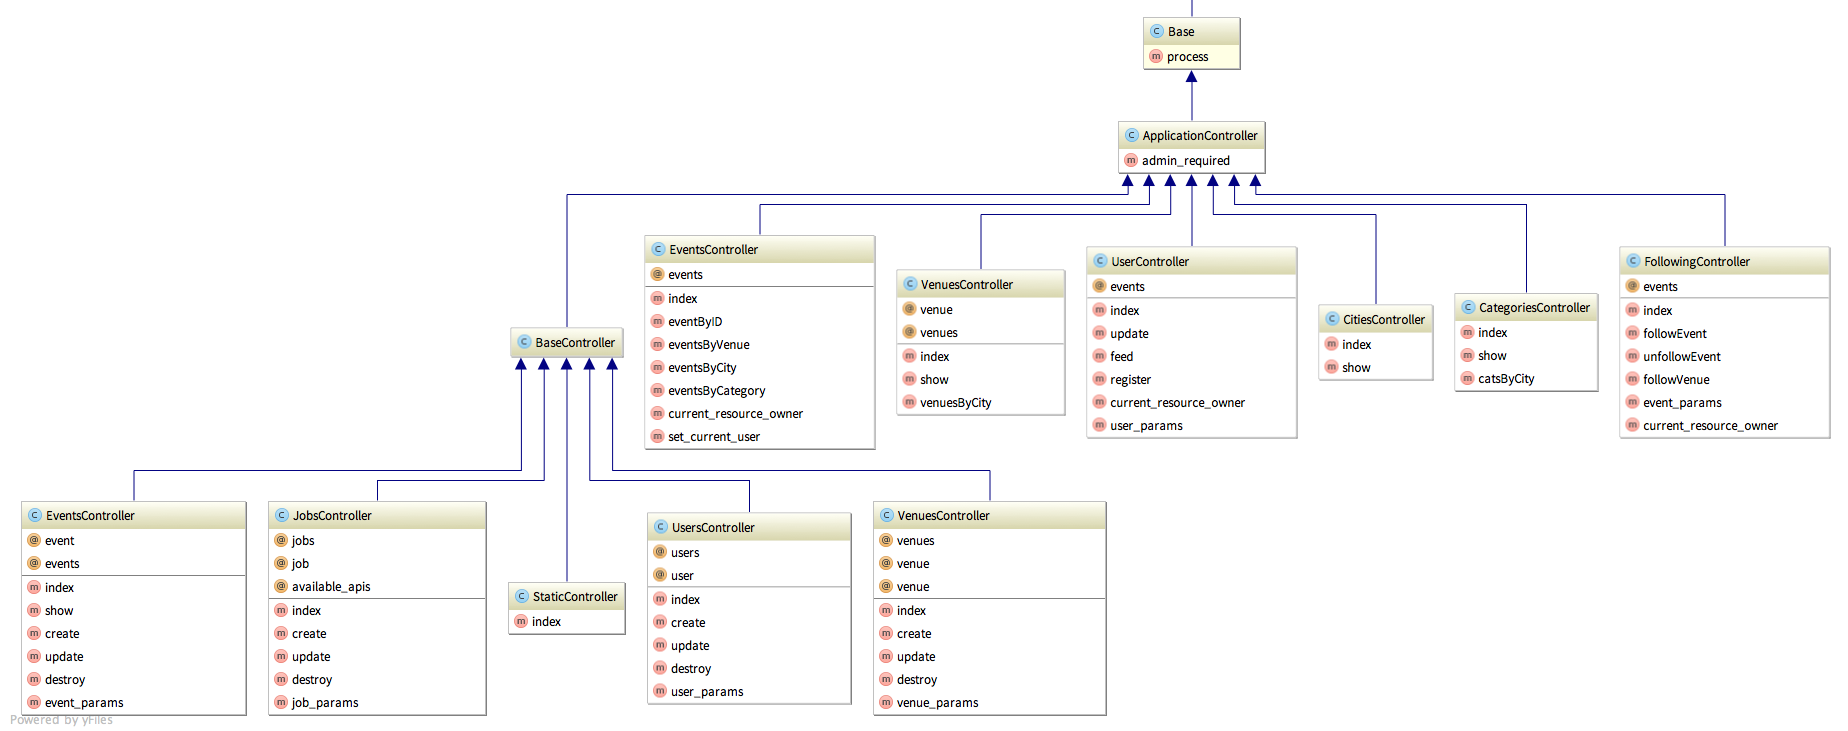
\includegraphics[width=1\textwidth,angle=90]{Images/controllers_crop}
				\label{fig:controllers}
			\end{figure}


	\section{iOS Application}

		\subsection{Development tools}
			To develop in iOS you are required to use Apples own IDE XCode, version 5 is the latest and supports the latest version of iOS. XCode 5 includes a number of tools bundled with the IDE including the iOS Simulator and GIT Integration. Cocoa pods will also be used for package management and pulling in various libraries that will be used throughout the project. XCode 5 itself is a purpose built IDE for iOS applications and everything that was required came as standard and was used as a one stop solution for the development of the mobile application. 

		\subsection{Wireframes}
			The main application will consist of 2 main views these being a list of events with some filter applied and the event details themselves. Figure \ref{fig:wireframes} depicts a rough outline of where elements will be positioned and the possible interactions a user can undertake. Figure \ref{fig:multi-events} shows the various different ways I could present the data using the iOS' table view to show list events happening, the list of events screen will be re-usable and able to show a list of events with a wide range of filters applied to it. The filters applied will be dependant on how the user access the list view be it through the `Discover' tab or the `My Feed' tab. 

			The wireframes show the 3 key different screens, the first being the `My Feed' tab  this tab is used to show the users personalised feed, this will utilise the list view for the events and then when an event is selected it will show the user the selected event using the individual event view. The second is the `Discover' tab this will be used to be able to select events from a particular city, it will then give you the option to select a particular category or venue to see relevant events to the selector chosen. The third is the `My Profile' tab this will be where you can see your information potentially change it and view the events you are following, this will also present you with the option to `unfollow' these events as well.

			\begin{figure}[H]
				\centering
				\caption{Basic wireframes and design choices for the mobile application}
				\begin{minipage}{.5\linewidth}
					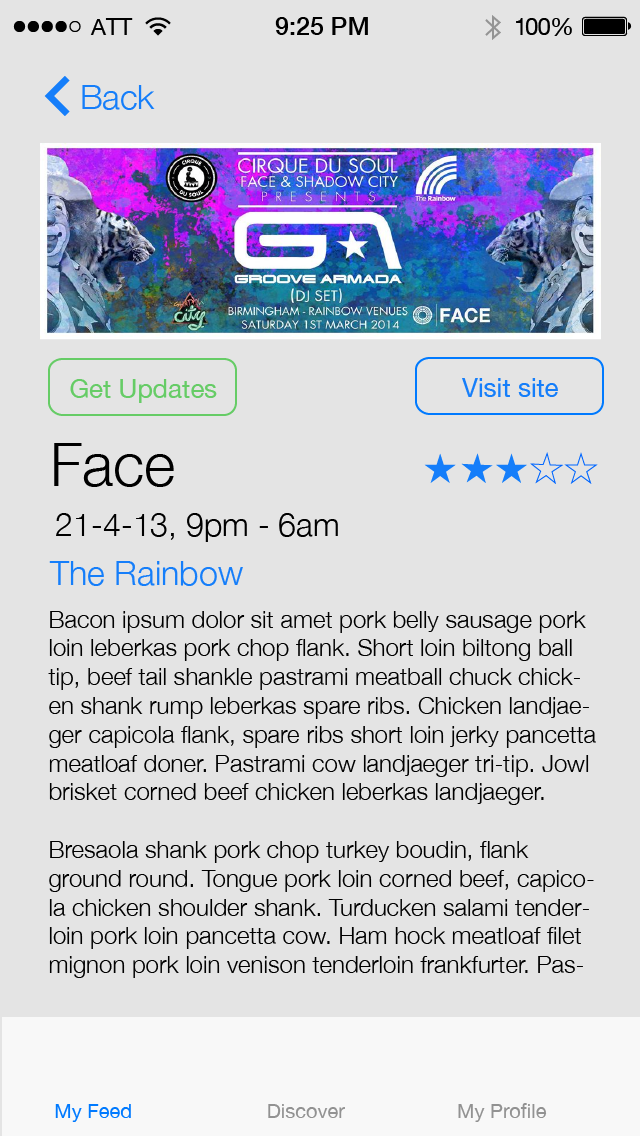
\includegraphics[width=0.9\textwidth]{Images/indiv-event}
					\caption{Individual event wireframe}
					\label{fig:indiv-event}
				\end{minipage}%
				\begin{minipage}{.5\linewidth}
					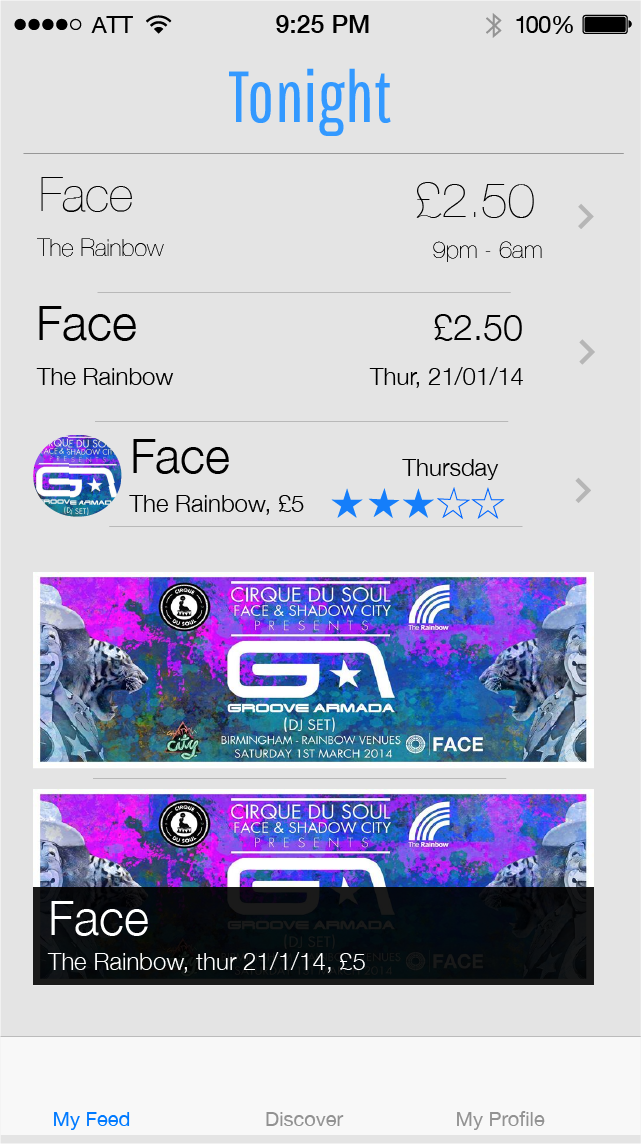
\includegraphics[width=0.9\textwidth]{Images/multi-events}
					\caption{List of events wireframe}
					\label{fig:multi-events}
				\end{minipage}
				\label{fig:wireframes}
			\end{figure}

		\subsection{Class diagrams}
			The majority of the application design was based on the delegation design pattern where actions and data are linked with the UI elements, and so the mobile application is a series of controllers where it retrieves information and outputs this into the UI. There will be a different controller for each screen that can be viewed as part of the application. Including this I will be using data classes to store and use the data pulled in from the server. Figure \ref{fig:ios-data} shows the 2 classes I will be using to keep the data retrieved from the API, these classes are simple data classes that have some functionality applied to them and allow for scope as the project develops. 

			\begin{figure}
				\centering
				\caption{Class diagram for the iOS data classes}
				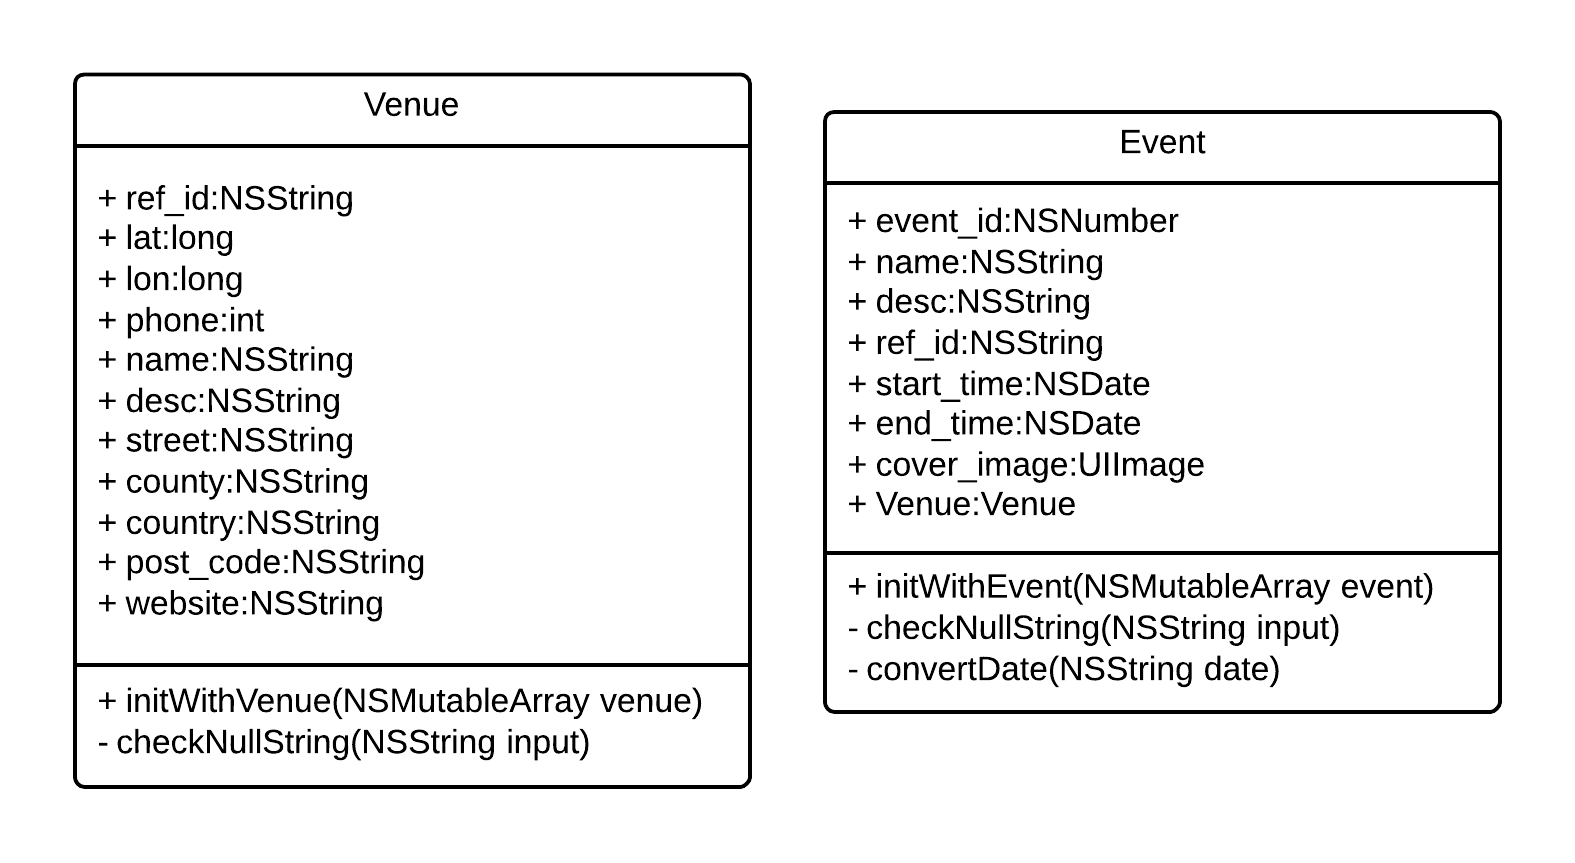
\includegraphics[width=0.6\linewidth]{Images/ios-data}
				\label{fig:ios-data}
			\end{figure}